\documentclass[14pt, a4paper]{extarticle}
\usepackage{GOST}
\usepackage{array}
\usepackage{verbatim}
\usepackage[detect-all]{siunitx}
\usepackage{amsmath}
\usepackage{amssymb}
\usepackage[utf8]{inputenc}
\usepackage{hyperref}
\usepackage{tempora}

\makeatletter
\renewcommand\@biblabel[1]{#1.}
\makeatother

\usepackage{listings}
\lstset{ 
	language=python,
	basicstyle=\small\sffamily, 
	numbers=left, 
	numberstyle=\tiny,
	stepnumber=1,
	numbersep=5pt,
	showspaces=false,            
	showstringspaces=false,      
	showtabs=false,             
	frame=single,            % рисовать рамку вокруг кода
	tabsize=4,      
	commentstyle=\color{green},
	keywordstyle=\color{blue}\textbf,
	numberstyle=\scriptsize\color{gray}, % the style that is used for the line-numbers
	rulecolor=\color{black},
	captionpos=t,
	breaklines=true,         % автоматически переносить строки 
	breakatwhitespace=false, % переносить строки по пробелу
	escapeinside={\#*}{*)} 
}


\usepackage{pgfplots}
\usepackage{filecontents}
\usetikzlibrary{datavisualization}
\usetikzlibrary{datavisualization.formats.functions}

\begin{document}
	
\begin{table}[ht]
	\centering
	\begin{tabular}{|c|p{400pt}|} 
		\hline
		\begin{tabular}[c]{@{}c@{}} 
\includegraphics[scale=1]{source/b_logo.jpg} \\\end{tabular} &
		\footnotesize\begin{tabular}[c]{@{}c@{}}\textbf{Министерство~науки~и~высшего~образования~Российской~Федерации}\\\textbf{Федеральное~государственное~бюджетное~образовательное~учреждение}\\\textbf{~высшего~образования}\\\textbf{«Московский~государственный~технический~университет}\\\textbf{имени~Н.Э.~Баумана}\\\textbf{(национальный~исследовательский~университет)»}\\\textbf{(МГТУ~им.~Н.Э.~Баумана)}\\\end{tabular}  \\
		\hline
	\end{tabular}
\end{table}
\noindent\rule{\textwidth}{4pt}
\noindent\rule[14pt]{\textwidth}{1pt}
\hfill 
\noindent
\makebox{ФАКУЛЬТЕТ~}%
\makebox[\textwidth][l]{\underline{~«Информатика и системы управления»~~~~~~~~~~~~~~~~~~~~~~~~~~~~~~~~~}}%
\\
\noindent
\makebox{КАФЕДРА~}%
\makebox[\textwidth][l]{\underline{~«Программное обеспечение ЭВМ и информационные технологии»~}}%
\\

\begin{center}
	\vspace{1.5cm}
	{\bf\huge Отчёт\par}
	{\bf\Large по лабораторной работе № 6\par}
	\vspace{0.7cm}
\end{center}


\noindent
\makebox{\large{\bf Название:}~~~}
\makebox[\textwidth][l]{\large\underline{~Муравьиный алгоритм. Решение задачи коммивояжера.~}}\\

\noindent
\makebox{\large{\bf Дисциплина:}~~~}
\makebox[\textwidth][l]{\large\underline{~Анализ алгоритмов~~~~~~~~~~~~~~~~~~~~~~~~~~}}\\

\vspace{1.5cm}
\noindent
\begin{tabular}{l c c c c c}
	Студент      & ~ИУ7-55Б~               & \hspace{2.5cm} & \hspace{2cm}                 & &  Д.О. Склифасовский \\\cline{2-2}\cline{4-4} \cline{6-6} 
	\hspace{3cm} & {\footnotesize(Группа)} &                & {\footnotesize(Подпись, дата)} & & {\footnotesize(И.О. Фамилия)}
\end{tabular}

\noindent
\begin{tabular}{l c c c c}
	Преподователь & \hspace{5cm}   & \hspace{2cm}                 & & ~~~~~~Л.Л. Волкова~~~~~~\\\cline{3-3} \cline{5-5} 
	\hspace{3cm}  &                & {\footnotesize(Подпись, дата)} & & {\footnotesize(И.О. Фамилия)}
\end{tabular}

\vspace{0.6cm}
\begin{center}	
	\vfill
	\large \textit {Москва, 2020}
\end{center}

\thispagestyle {empty}
\pagebreak

% СОДЕРЖАНИЕ 
\clearpage
\tableofcontents

% ВВЕДЕНИЕ
\clearpage
\section*{Введение}
\addcontentsline{toc}{section}{Введение}
Задача коммивояжёра — одна из самых известных задач комбинаторной оптимизации, заключающаяся в поиске самого выгодного маршрута, проходящего через указанные города хотя бы по одному разу с последующим возвратом в исходный город.\par
Целью данной лабораторной работы является создание приложения для наглядного представления работы муравьиного алгоритма.\par
Задачи данной лабораторной работы:
\begin{enumerate}
	\item[1)] изучить существующие методы решения задачи;
	\item[2)] реализовать алгоритм полного перебора и муравьиный алгоритм;
	\item[3)] сравнить время работы этих алгоритмов.
\end{enumerate} 

% АНАЛИТИЧЕСКИЙ РАЗДЕЛ
\clearpage
\section{Аналитический раздел}
Задача коммивояжера занимает особое место в комбинаторной оптимизации и исследовании операций. Исторически она была одной из тех задач, которые послужили толчком для развития этих направлений. С точки зрения приложений, она не представляет интерес. Куда важнее её обобщения для транспорта и логистики, когда несколько транспортных средств ограниченной грузоподъемности должны обслуживать клиентов, посещая их в заданные временные окна. 
\subsection{Общие сведения}
В задаче коммивояжера рассматривается городов и матрица попарных расстояний между ними. Требуется найти такой порядок посещения городов, чтобы суммарное пройденное расстояние было минимальным, каждый город посещался ровно один раз и коммивояжер вернулся в тот город, с которого начал свой маршрут. Другими словами, во взвешенном полном графе требуется найти гамильтонов цикл минимального веса.\par
\subsection{Алгоритм полного перебора}
Под полным перебором понимается методика разрешения задач математики путем рассмотрения всех возможных вариантов. Уровень сложности при полном переборе напрямую связан с количеством допустимых решений задачи. В случае, когда область решений огромна, время полного перебора может исчисляться десятками и даже сотнями лет, и при этом итоговый результат возможно ещё не будет найден. Все задачи класса NP могут быть решены при помощи полного перебора.
\subsection{Муравьиный алгоритм}
Идея муравьиного алгоритма - моделирование поведения муравьев, связанное с их способностью быстро находить кратчайший путь от муравейника к источнику пищи и адаптироваться к изменяющимся условиям, находя кратчайший путь.\par
С учетом особенности задачи коммивояжера, можно описать правила поведения муравьев при выборе пути:
\begin{enumerate}
	\item[1)] муравьи имеют собственную "память"\ - у муравья уже есть список посещенных городов;
	\item[2)] муравьи обладают "зрением"\ - видимость есть эвристическое желание посетить город $j$, если муравей находится в городе $i$;\par
	\begin{equation*}
		\eta_{ij} = \frac{1}{D_{ij}}
	\end{equation*}
	\item[3)] муравьи обладают "обонянием"\ - они могут улавливать след феромона, подтверждающий желание посетить город $j$ из города $i$ на основании опыта других муравьев.
\end{enumerate}
На этом основании можно сформулировать вероятностно-пропорциональное правило, определяющее вероятность перехода k-ого муравья из города $i$ в город $j$:
\begin{equation*}
	\left\{ \begin{array}{l | l}
		P_{ij,k}(t)=\frac{[\tau_{ij}(t)]^\alpha*[\eta_{ij}]^\beta}{\sum_{l\in J_{ik}}[\tau_{il}(t)]^\alpha * [\eta_{il}]^\beta}, & j \in J_{i,k};\\
		P_{ij,k}(t) = 0, & j \not\in J_{i,k}
	\end{array} \right.
\end{equation*}
Где $\alpha,\beta$ - параметры, задающие веса следа феромона.\par
Пройдя ребро $(i,j)$, муравей откладывает на нем некоторое количество феромона. Пусть $T_k(t)$ есть маршрут, пройденный муравьем $k$ к моменту времени t, а $L_k(t)$ - длина этого маршрута. Пусть $Q$ - параметр, имеющий значение порядка длины оптимального пути. Тогда откладываемое количество феромона может быть задано в виде:
\begin{equation*}
	\Delta\tau_{ij,k}(t) = \left\{ \begin{array}{l | l}
		\frac{Q}{L_k(t)}, & (i,j)\in T_k(t)\\
		0, & (i,j)\not\in T_k(t)
	\end{array} \right.
\end{equation*}
Правила внешней среды в первую очередь определяют испарение феромона. Пусть $p\in [0,1]$ есть коэффициент испарения, тогда правило испарения имеет вид:
\begin{equation*}
	\tau_{ij}(t+1) = (1-p)\tau_{ij}(t)+\Delta\tau_{ij}(t); \Delta\tau_{ij}(t) = \sum_{k=1}^{m}\Delta\tau_{ij,k}(t),
\end{equation*}
где m - количество муравьев в колонии.
\subsection{Вывод}
В данном разделе представлены общие сведения задачи коммивояжера, описание алгоритмов полного перебора и муравьиный.

\clearpage
\section{Конструкторский раздел}
В данном разделе представлены схемы алгоритмов полного перебора и маравьиный.
\subsection{Алгоритм полного перебора}
\textbf{Функция GetRoute}\par
На рисунке 1 показана основная функция GetRoute.
\begin{figure}[h!]
	\centering
	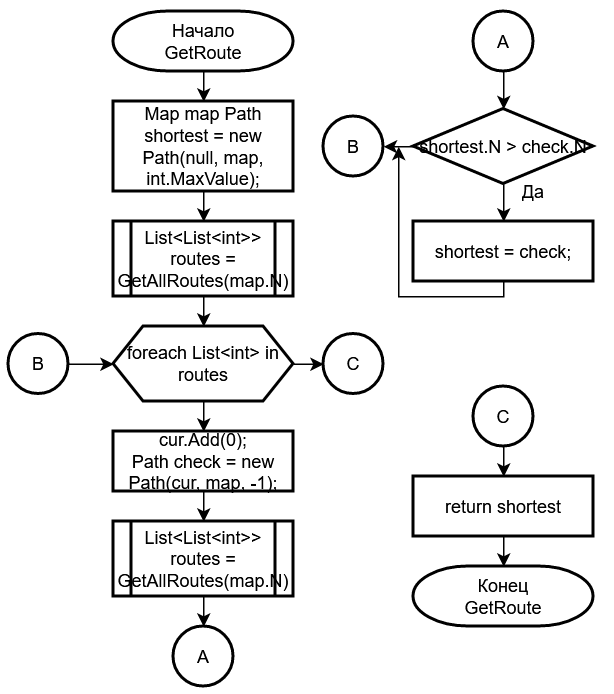
\includegraphics[scale=1]{source/GetRoute.png}
	\caption{Функция GetRoute}
\end{figure}	
\newpage
\textbf{Функция GetAllRoutes}\par
На рисунке 2 показана функция GetAllRoutes.
\begin{figure}[h!]
	\centering
	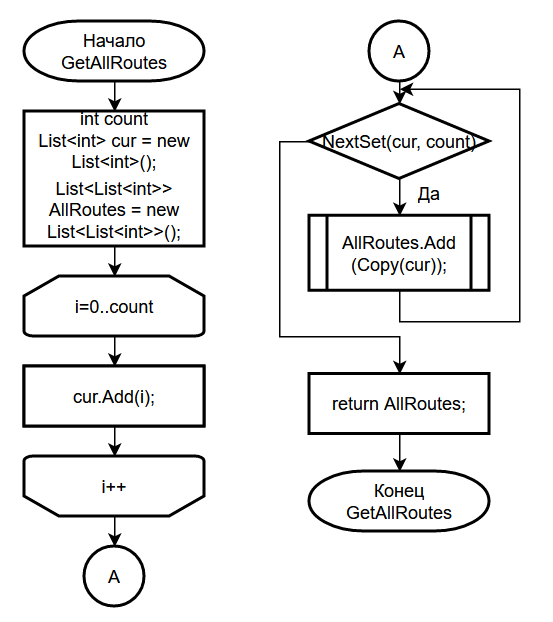
\includegraphics[scale=1]{source/GetAllRoutes.png}
	\caption{Функция GetAllRoutes}
\end{figure}
\newpage
\textbf{Функция NextSet}\par
На рисунке 3 показана функция NextSet.
\begin{figure}[h!]
	\centering
	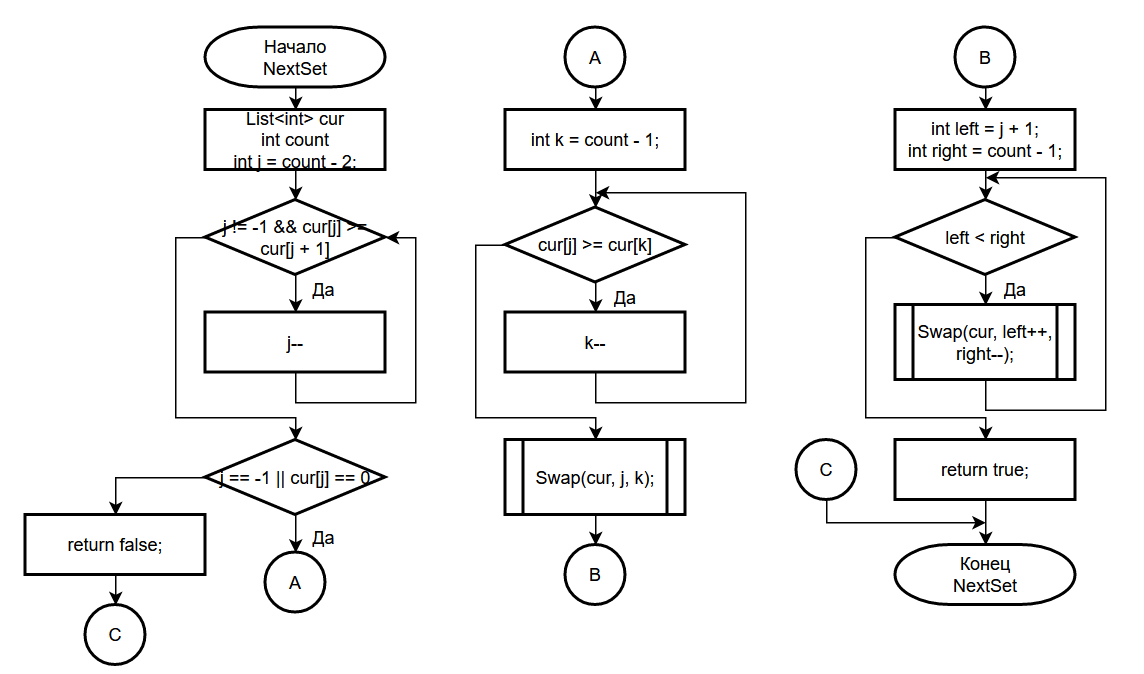
\includegraphics[width=\linewidth]{source/NextSet.png}
	\caption{Функция NextSet}
\end{figure}
\newpage
\subsection{Муравьиный алгоритм}
На рисунке 4 показан муравьиный алгоритм.
\begin{figure}[h!]
	\centering
	\includegraphics[scale=1]{source/Ant.png}
	\caption{Муравьиный алгоритм}
\end{figure}
\subsection{Вывод}
В данном разделе были разработаны алгоритмы полного перебора и муравьиный.

\newpage
\section{Технологический раздел}
В данном разделе даны общие требования к программе, средства реализации и сама реализация алгоритмов.
\subsection{Общие требования}
\textbf{Требования к программе}
\begin{enumerate}
	\item[1)] алгоритм полного перебора должен возвращать кратчайший путь;
	\item[2)] работа программы должна быть корректна.
\end{enumerate}
В качестве языка программирования был выбран C\#\hyperref[literature]{[1]}, так как я знаком с данным языком программирования, имею представление о способах тестирования программы.\par
Средой разработки Visual Studio.\hyperref[literature]{[2]}\par 
Для замеров процессорного времени используется функция $Stopwatch$.\hyperref[literature]{[3]}\hyperref[literature]{[4]}\par
\subsection{Сведения о модулях программы}
Программа состоит из:
\begin{enumerate}
	\item[1)] Program.cs - главный файл программы, в котором располагается точка входа в программу;
	\item[2)] BruteForce.cs - файл класса алгоритма полного перебора;
	\item[3)] AntAlgorithm.cs - файл класса муравьиного алгоритма;
	\item[4)] Map.cs - файл класса, содержащего матрицу смежности;
	\item[5)] Path.cs - файл класса, содержащий путь и методы для работы с ним.
\end{enumerate}
\subsection{Листинг кода программы}
\subsection{Алгоритм полного перебора}
В листинге 1 представлена основная функция GetRoute.
\begin{lstlisting}[caption=GetRoute]
public static Path GetRoute(Map map)
{
	Path shortest = new Path(null, map, int.MaxValue);
	foreach (List<int> cur in GetAllRoutes(map.N))
	{
		cur.Add(0);
		Path check = new Path(cur, map, -1);
		check.GetDistance();
		if (shortest.N > check.N)
			shortest = check;
	}
	return shortest;
}
\end{lstlisting}
В листинге 2 представлена функция GetAllRoutes.
\begin{lstlisting}[caption=GetAllRoutes]
private static List<List<int>> GetAllRoutes(int count)
{
	List<List<int>> AllRoutes = new List<List<int>>();
	List<int> cur = new List<int>();
	for (int i = 0; i < count; i++)
		cur.Add(i);
	while (NextSet(cur, count))
		AllRoutes.Add(Copy(cur));
	return AllRoutes;
}
\end{lstlisting}
В листинге 3 представлена функция NextSet.
\begin{lstlisting}[caption=NextSet]
private static bool NextSet(List<int> cur, int count)
{
	int j = count - 2;
	while (j != -1 && cur[j] >= cur[j + 1]) j--;
	if (j == -1 || cur[j] == 0)
		return false;
	int k = count - 1;
	while (cur[j] >= cur[k]) 
		k--;
	Swap(cur, j, k);
	int left = j + 1; 
	int right = count - 1;
	while (left < right)
		Swap(cur, left++, right--);
	return true;
}
\end{lstlisting}
\subsection{Муравьиный алгоритм}
В листинге 4 представлен муравьиный алгоритм.
\begin{lstlisting}[caption=NextSet]
public static Path GetRoute(Map map, int maxTime, double alpha, double beta, double Q, double pho)
{
	Random r = new Random();
	
	Path shortest = new Path(null, map, int.MaxValue);
	
	int count = map.N;
	double[,] pher = InitPheromone(0.1, count);
	
	List<Ant> ants = null;
	
	for (int time = 0; time < maxTime; time++)
	{
		ants = InitAnts(map);
		for (int i = 0; i < count - 1; i++)
		{
			double[,] deltaPher = InitPheromone(0, count);
			foreach (Ant ant in ants)
			{
				int curTown = ant.LastVisited();
				
				double sum = 0;
				for (int town = 0; town < count; town++)
				{
					if (!ant.IsVisited(town))
					{
						double tau = pher[curTown, town];
						double eta = 1 / map[curTown, town];
						sum += Math.Pow(tau, alpha) * Math.Pow(eta, beta);
					}
				}
				
				double check = r.NextDouble();
				int newTown = 0;
				for (; check > 0; newTown++)
				{
					if (!ant.IsVisited(newTown))
					{
						double tau = pher[curTown, newTown];
						double eta = 1 / map[curTown, newTown];
						double chance = Math.Pow(tau, alpha) * Math.Pow(eta, beta) / sum;
						check -= chance;
					}
				}
				newTown--;
				ant.VisitTown(newTown);
				deltaPher[curTown, newTown] += Q / map[curTown, newTown];
			}
			for (int k = 0; k < count; k++)
				for (int t = 0; t < count; t++)
					pher[k, t] = (1 - pho) * pher[k, t] + deltaPher[k, t];
		}
		foreach (Ant ant in ants)
		{
			ant.VisitTown(ant.Start);
			
			if (ant.GetDistance() < shortest.N)
				shortest = ant.GetPath();
		}
	}
	return shortest;
}
\end{lstlisting}
\subsection{Вывод}
В данном разделе были представлены общие требования к программе, сведения о модулях и листинги алгоритмов полного перебора и муравьиный.

\clearpage
\section{Экспериментальный раздел}
В данном разделе приведен анализ времени работы алгоритмов.
\subsection{Замер времени}
Проводится замер времени при разных размерах матрица смежности (разном количестве вершин графа). На рисунке 5 показан результат замеров.
\begin{figure}[h!]
	\centering
	\begin{tikzpicture}[object/.style={thin,double,<->}]
		
		\begin{axis}[
			axis lines = left,
			xlabel = $\textit{Размер матрицы смежности}$,
			ylabel = {$\textit{Время (тики)}$},
			legend pos=north west,
			ymajorgrids=true
			]
			\addplot[color=red] table[x index=0, y index=1] {source/Brute.dat}; 
			\addplot[color=orange] table[x index=0, y index=1] {source/Ant.dat};
			
			\addlegendentry{Полный перебор}
			\addlegendentry{Бинарный поиск}
			
		\end{axis}
	\end{tikzpicture}
	
	\caption{Результаты замеров процессорного времени.}
	\label{Test1}
\end{figure}\par
Можно увидеть, что муравьиный алгоритм намного быстрее, чем алгоритм полного перебора, при большом размере графа. До 7 вершин алгоритм полного перебора работает практически одинаково, а далее начинает резко увеличиваться время работы.
\subsection{Параметризация}
Проводится выборка лучших сочетаний значений $\alpha, \beta, \rho$. На рисунке 6 можно увидеть результат тестирования.
\begin{figure}[h!]
	\centering
	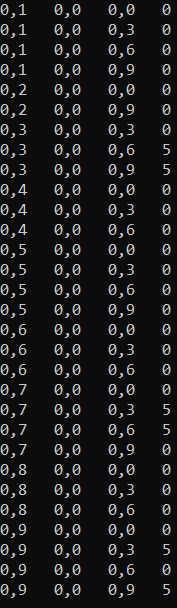
\includegraphics[scale=1]{source/test.png}
	\caption{Результат тестирования}
\end{figure}
\subsection{Вывод}
По результатам тестирования можно сделать вывод, что на небольших размерах графа алгоритм полного перебора работает быстрее, но на больших размерах он во много раз медленнее муравьиного алгоритма.\par
Наиболее правильные результаты получаются при $\alpha = 0.5..0.9$, $\beta = 0$.

\clearpage
\section*{Заключение}
\addcontentsline{toc}{section}{Заключение}
В ходе выполнения лабораторной работы было создано приложения для наглядного представления работы муравьиного алгоритма. Были выполнены следующие задачи:
\begin{enumerate}
	\item[1)] изучены существующие методы решения задачи;
	\item[2)] реализованы алгоритмы полного перебора и муравьиный алгоритм;
	\item[3)] были проведены эксперименты.
\end{enumerate}\par
При размерах графа больше 7-8 выгоднее использовать муравьиный алгоритм, так как он в несколько раз быстрее алгоритма полного перебора. Но не всегда муравьиный алгоритм дает минимальный результат.

\clearpage
\section*{Литература}
\addcontentsline{toc}{section}{Литература}
\begin{enumerate}
	\label{literature}
	\item  Документация по C\#. -URL: \href{https://docs.microsoft.com/ru-ru/dotnet/csharp/}{https://docs.microsoft.com/ru-ru/dotnet/csharp/} (дата обращения: 24.10.2020). -Текст: электронный.
	\item Документация по семейству продуктов Visual Studio. -URL:\par \href{https://docs.microsoft.com/ru-ru/visualstudio/?view=vs-2019}{https://docs.microsoft.com/ru-ru/visualstudio/?view=vs-2019 } (дата обращения: 01.10.2020). -Текст: электронный.
	\item Stopwatch Класс. -URL: \href{https://goo.su/2e99}{https://goo.su/2e99 } (дата обращения: 24.10.2020). -Текст: электронный.
	\item Под капотом у Stopwatch. -URL:  \href{https://habr.com/ru/post/226279/}{https://habr.com/ru/post/226279/} (дата обращения: 24.10.2020). Текст: электронный.
\end{enumerate}
\end{document}\par














